\documentclass{report}

\usepackage[italian]{babel} % Imposta la lingua italiana
\usepackage{tcolorbox}
\usepackage{forest}
\usepackage{dirtree} % Aggiungi il pacchetto dirtree
\usepackage{graphicx} % Aggiungi il pacchetto graphicx
\usepackage{pgfplots}
\usepackage{wrapfig}
\usepackage{amsmath}
\usepackage{circuitikz}
\usepackage{hyperref}
\hypersetup{
    colorlinks=true,
    linkcolor=black,
    filecolor=magenta,      
    urlcolor=cyan,
    pdftitle={Overleaf Example},
    pdfpagemode=FullScreen,
    }
\pgfplotsset{width=5cm,compat=1.9}

\renewcommand{\thefootnote}{\roman{footnote}}
% Definizione del nuovo ambiente 'important'
\newtcolorbox{important}[1][]{
  colback=yellow!10!white,
  colframe=red!50!black,
  title=Ricorda,
  #1
}
% Definizione del nuovo ambiente 'definition'
\newtcolorbox{definition}[1][]{
  colback=blue!10!white,
  colframe=blue!50!black,
  title=Definizione,
  #1
}
% Definizione del nuovo ambiente 'property'
\newtcolorbox{property}[1][]{
  colback=green!10!white,
  colframe=green!50!black,
  title=Proprietà,
  #1
}
\begin{document}

\begin{center}
  \vspace*{2cm}
  {\Huge Fisica sperimentale I \par}
  \vspace{1cm}
  
\includegraphics[width=0.5\textwidth]{logounibs.png}\par
  \vspace{1cm}
  {\Large Riccardo Rasori \par}
  \vspace{0.5cm}
  {\large A.A. 2024/2025 \par}
  \vspace{2cm}
\end{center}

\tableofcontents % Aggiungi l'indice

\chapter{Introduzione}

\section{Il metodo scientifico}
La natura è complessa $\rightarrow$ per capirla si fanno esperimenti\\
Es. Tolta l'aria (nel vuoto) tutti i corpi cadono in maniera uguale
\\
$\rightarrow$ Gli esperimenti formulano una teoria\\
$\rightarrow$ La fisica usa il linguaggio matematico per le teorie e le leggi\\
\section{Grandezze fisiche}
\begin{definition}
  \textbf{Misurazione}: si associa un numero (misura) a una grandezza fisica. Associa anche la sua attendibilità (errore).\\
  Deve essere non ambigua e riproducibile.
\end{definition}
\begin{definition}
  \textbf{Grandezza fisica}: è definita in relazione al procedimento/strumento utilizzato per misurare.\\
  Non tutte le grandezze sono indipendenti (velocità $\frac{m}{s}$).
\end{definition}
\dirtree{%
  .1 Sistema Internazionale.
  .2 Tempo (s).
  .2 Lunghezza (m).
  .2 Massa (kg).
  .2 Quantità di materia (mol).
  .2 Temperatura (K).
  .2 Intensità di corrente elettrica (A).
  .2 Intensità luminosa (cd).
}
\subsection{Tempo}
Grandezza fisica misurata con l'orologio.\\
Si usa l'orologio atomico basato sulla frequenza di una transizione iperfine all'atomo di $^{133}Cs$ (Cesio)
\begin{definition}
  \textbf{Secondo}: tempo che ci mette la luce emessa da $^{133}Cs$ per fare $9.192.631.770$ vibrazioni.
\end{definition}
\subsection{Lunghezza}
Si usa il regolo per misurarla
\begin{definition}
  \textbf{Metro}: distanza percorsa dalla luce nel vuoto in $\frac{1}{299.792.458}$ di secondo.
\end{definition}
\subsection{Massa}
\begin{definition}
  \textbf{Massa}: grandezza fisica misurata con bilancia a due bracci.
\end{definition}
Campione di riferimento: kg $\rightarrow$ cilindro di platino-iridio per definire la massa
\section{La notazione scientifica}
\dirtree{%
.1 Vantaggi.
.2 È formalmente compatta.
.2 È evidente l'\underline{ordine di grandezza} $\rightarrow$ {Potenza di 10 con cui è espresso il numero}.
.2 È evidente la precisione con cui è noto il valore numerico $\rightarrow$ L'incertezza è espressa dal suo errore\\ {Es. $l=(3,5\pm0,1)m$}.
}
L'errore ci dice quante cifre significative usare per rappresentare una grandezza\\
Es. $(4,5397\pm0,21)*10^{3} \leftarrow$ se già la prima cifra è incerta per l'errore, non ha senso precisare tutto quello che c'è dopo (397)
\\
$\rightarrow$ va scritto $(4,54\pm0,21)*10^{3}$
\subsection{Num cifre significative}
3m $\rightarrow$ per l'errore può essere $3\pm0,1$ m (2, 3 o 4)\\
3,0m $\rightarrow$ per l'errore può essere $3,0\pm0,1$ m (2,9; 3,0; 3,1)\\
0,003m $\leftarrow$ 1 cifra significativa\\
0,0030m $\leftarrow$ 2 cifre significative\\

\subsubsection{Addizione}
\begin{center}

  \begin{tabular}{r}
    18,0      \\
    + 0,0039  \\
    + 0,00002 \\
    \hline
    18,00392  \\
    = 18,0
  \end{tabular}

\end{center}\footnote{deve contenere un numero di cifre significative uguale a quello del numero con incertezza maggiore}

\subsubsection{Moltiplicazione}
Il risultato \underline{di norma} deve contenere tante cifre significative quante ne sono contenute nel fattore con meno cifre significative
\begin{center}

  \begin{tabular}{r}
    Es:     \\
    2,21    \\
    $* 0,3$ \\
    \hline
    0,663   \\
    = 0,7
  \end{tabular}
\end{center}
Es. $12,4*84=1041,6=1,04*10^{3}$
\subsubsection{Divisione}
Vale la stessa regola della moltiplicazione\\
Es. $14,28/0,714=20=20,0$ oppure $2,0*10^{1}$\\
Es. $0,032/0,004=8=0,8*10^{1}$\\
Es: $9,83/9,3$\footnote{2 cifre, ma l'incertezza è circa dell'1\%}$=1,05698924731=1,06$\footnote{Se avessi scritto 1,1 l'incertezza era circa del 10\%, quindi metto 1,06 e l'incertezza rimane circa 1\%}\\
\section{Meccanica}
\begin{itemize}
  \item \textbf{Cinematica}: studio del moto indipendente dalle cause
  \item \textbf{Dinamica}: studio del moto in relazione alle forze agenti
  \item \textbf{Statica}: studio del moto in assenza di forze
\end{itemize}
\subsection{Cinematica}
\begin{itemize}
  \item Si studia un corpo puntiforme (particella) in cui è incentrata la massa
  \item Lo studiamo in modo unidimensionale (si muove solo in una direzione) (moto rettilineo)
        \begin{itemize}
          \item Posizione
          \item Spostamento
          \item Velocità
          \item Accelerazione
        \end{itemize}
  \item In natura esistono corpi puntiformi (elettroni)
        \begin{itemize}
          \item Hanno raggio $<2*10^{-20}$ m
        \end{itemize}
\end{itemize}
\subsubsection{Moto}
\begin{itemize}
  \item Il suo concetto è relativo
        \begin{itemize}
          \item Per un osservatore un oggetto potrebbe essere in movimento, per un altro potrebbe essere fermo
        \end{itemize}
  \item \underline{Sistema di riferimento}
        \begin{itemize}
          \item Definisce la posizione di un corpo
          \item Assi x y z
          \item In cinematica il sistema di rif. è arbitrario (1,2,3 dimensioni)
          \item La \underline{posizione} p la coordinata lungo l'asse della particella
          \item Lo \underline{spostamento} è la differenza tra il valore della pos. finale e quella iniziale\\$\Delta x=x_2-x_1$
          \item Conviene descrivere il moto con il variare della posizione in funzione del tempo\\Ho la funzione $x(t)$ dove il tempo è la variabile indipendente\\\begin{tikzpicture}
                  \begin{axis}[
                      axis x line=middle,
                      axis y line=middle,
                      enlargelimits,
                      xtick={1,2,3,4},
                      xlabel={$t$},
                      ylabel={},
                      ytick=\empty,
                      samples=100,
                      grid=major
                    ]
                    % Disegna la curva interpolata
                    \addplot[smooth, tension=0.8, thick, blue] coordinates {
                        (0,-2) (2,-1) (3,1) (4,2)
                      };

                    % Disegna i punti con cerchi vuoti
                    \addplot[only marks, mark=o, mark size=3pt] coordinates {
                        (0,-2) (2,-1) (3,1) (4,2)
                      };
                  \end{axis}
                \end{tikzpicture}
          \item La velocità è quanto rapidamente si muove la particella
                \begin{itemize}
                  \item Velocità vettoriale media\\È il rapporto tra lo spostamento $\Delta x$ che si verifica in un certo intervallo $\Delta t$ e l'intervallo stesso\\$\overline{v}=\frac{\Delta x}{\Delta t}=\frac{x_2(t_2)-x_1(t_1)}{t_2-t_1}[\frac{m}{s}]$\\$[\overline{v}]=[LT^{-1}]$\\\begin{tikzpicture}
                          \begin{axis}[
                              axis x line=middle,
                              axis y line=middle,
                              enlargelimits,
                              xtick={1,2,3,4},
                              xlabel={$t$},
                              ylabel={},
                              ytick=\empty,
                              samples=100,
                              grid=major
                            ]

                            % Disegna la curva interpolata
                            \addplot[smooth, tension=0.8, thick, blue] coordinates {
                                (1,-4) (3,0)  (4,2)
                              };

                            % Disegna i punti con cerchi vuoti
                            \addplot[only marks, mark=o, mark size=3pt] coordinates {
                                (1,-4) (3,0)  (4,2)
                              };

                            % Disegna la retta secante (velocità media tra due punti)
                            \addplot[domain=0.5:4.5, thick, green] {1.5*x - 4};

                          \end{axis}
                        \end{tikzpicture}
                        \\
                        Può succedere che la particella si muova e che torni nello stesso punto:
                        \begin{itemize}
                          \item lo spostamento è 0 $\Rightarrow$ la velocità vettoriale media è 0
                        \end{itemize}
                  \item Velocità scalare media\\$\overline{u}=\frac{l}{\Delta t}[m/s]$\\$[\overline{u}]=[LT^{-1}]$
                  \item Velocità istantanea\\
                        \begin{definition}
                          Limite della velocità vettoriale media quando $\Delta t$ tende a 0
                        \end{definition}$v(t)=\lim_{\Delta t\to0}\frac{\Delta x}{\Delta t}=\lim_{t \to t_1}\frac{x(t)-x(t_1)}{t-t_1}=\lim_{\Delta t\to0}\frac{x(t+\Delta t)-x(t)}{\Delta t}\Rightarrow v(t)=\frac{dx(t)}{dt}\rightarrow$ è la derivata prima di x(t) rispetto al tempo t\\
                        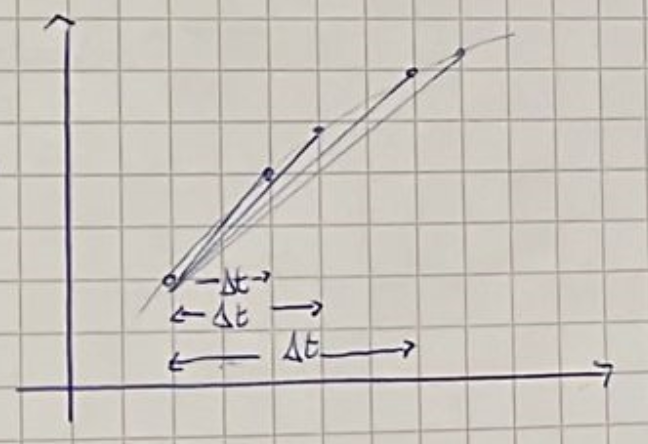
\includegraphics[scale=0.5]{grafico3.png}
                \end{itemize}
          \item Esempi di moti
                \begin{itemize}
                  \item Particella con velocità costante\\$x(t)=A+Bt$\\Velocità istantanea\\$v(t)=\frac{dx}{dt}=\frac{d}{dt}(A+Bt)=0+B$
                  \item Particella accelerata uniformemente
                \end{itemize}
          \item Accelerazione media o istantanea
                \begin{itemize}
                  \item Media: rapporto tra la variazione della velocità della particella in un $\Delta t$ e l'intervallo stesso\\$\overline{a}=\frac{\Delta v}{\Delta t}=\frac{v_2(t_2)-v_1(t_1)}{t_2-t_1}$\\$[\overline{a}]=[\frac{LT^{-1}}{T}]=[LT^{-2}]\rightarrow[\frac{m}{s^2}]$
                  \item Istantanea:\\$a(t)=\lim_{\Delta t\to0}\frac{\Delta v}{\Delta t}=\lim_{t\to t_1}\frac{v(t)-v(t_1)}{t-t_1}=\lim_{\Delta t\to0}\frac{v(t+\Delta t)-v(t)}{\Delta t}=\frac{dv(t)}{dt}=\frac{d^2xt}{dt^2}\rightarrow $ è la derivata seconda di x(t) rispetto al tempo t
                  \item Accelerazione e velocità concordi
                        \begin{itemize}
                          \item Parlo di accelerazione se la velocità aumenta
                          \item Parlo di decelerazione se la velocità diminuisce
                        \end{itemize}
                        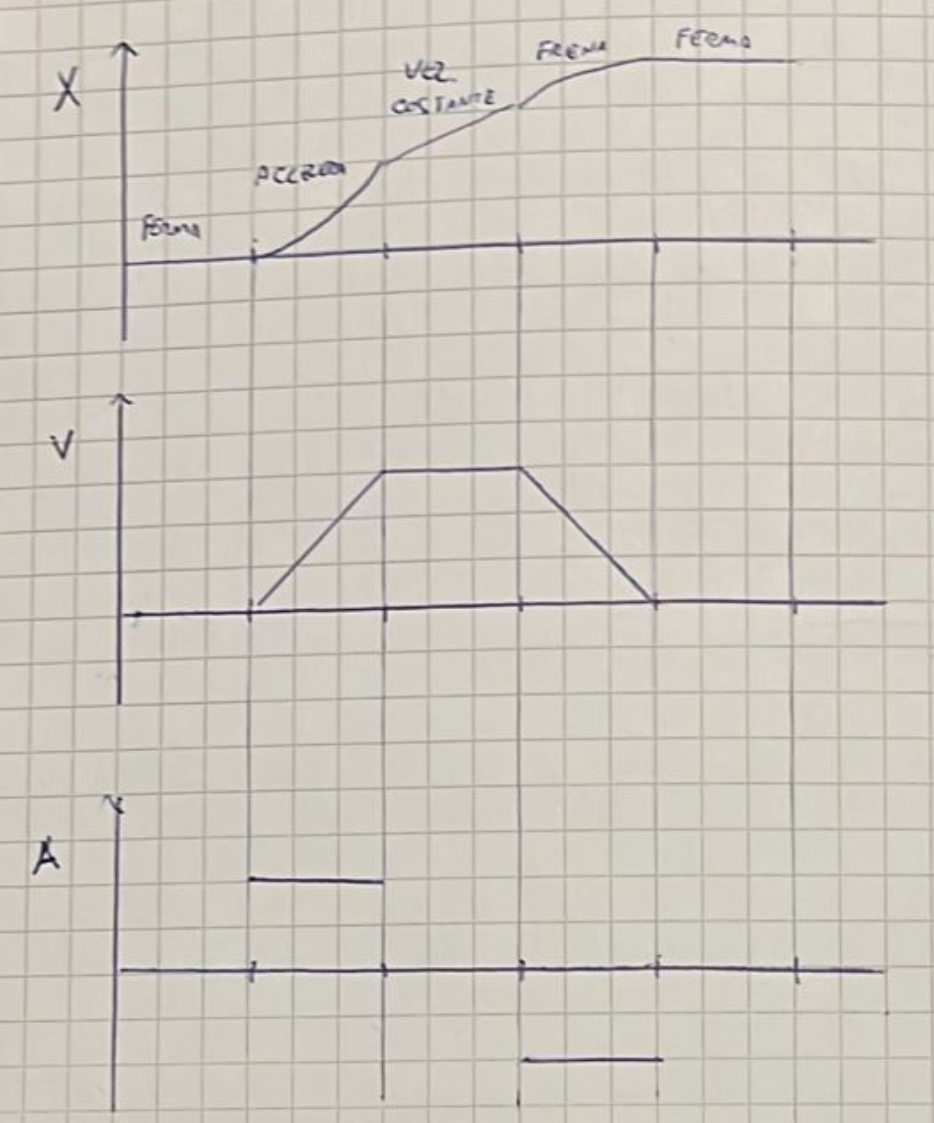
\includegraphics[scale=0.5]{grafico4.png}
                \end{itemize}
          \item Accelerazione costante
                \begin{itemize}
                  \item Trovo la velocità\\a(t)=costante e poniamo per semplicità $t_0=0$\\$a=\overline{a}=\frac{\delta v}{\delta t}=\frac{v-v_0}{t-0}\Rightarrow v(t)=v_0+a*t (1)$
                        \begin{center}
                          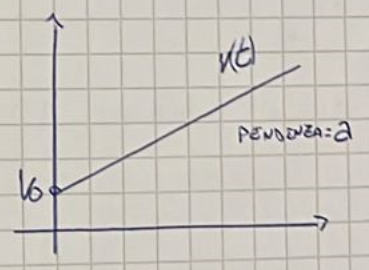
\includegraphics[scale=0.5]{grafico5.png}
                        \end{center}
                  \item Trovo la posizione\\
                        \begin{equation}
                          \begin{cases}
                            \overline{v}=\frac{1}{2}(v_0+v)=\frac{1}{2}(v_0+v_0+a*t)=v_0+\frac{1}{2}a*t \\
                            \overline{v}=\frac{\delta x}{\delta t}=\frac{x-x_0}{t-0}
                          \end{cases}
                        \end{equation}
                        $\Rightarrow x(t)=x_0+v_0*t+\frac{1}{2}a*t^2$ (2)\\
                        Posso conoscere dove si trova la particella a patto di sapere le condizioni iniziali di tempo e moto della particella\begin{center}
                          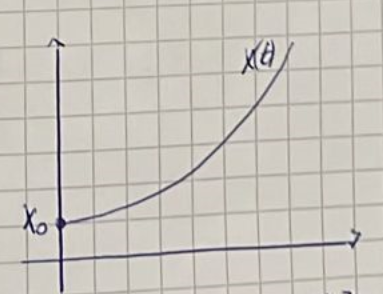
\includegraphics[scale=0.5]{grafico6.png}
                        \end{center}
                \end{itemize}
                Posso ricavare altre equazioni
                \begin{itemize}
                  \item eliminando t da (1) e (2)\\$v^2(x)=v_0^2+2a(x-x_0) (3)$
                  \item eliminando a da (1) e (2)\\$x(t)=x_0+\frac{v_0+v}{2}t (4)$
                  \item eliminando $v_0$ da (1) e (2)\\$x(t)=x_0+v(t)-\frac{1}{2}a(t^2) (5)$
                \end{itemize}
                La (1) e la (2) sono le più importanti, da sapere a memoria\\
                Mostriamo come a questi risultati si può arrivare anche con le derivate\\
                $a=\frac{dv}{dt}\Rightarrow dv=a*dt\Rightarrow \int_{x_0}^{x}dx=\int_{0}^{t}vdt=\int_{0}^{t}(v_0+a*t)dt \Rightarrow x-x_0=v_0*t+\frac{1}{2}a*t^2 \Rightarrow x=x_0+v_0*t+\frac{1}{2}a*t^2$\\
                Se al posto di $t_0$ avesso un t qualunque uso $t-t_0$\\
        \end{itemize}
  \item Moto di caduta libera\\In assenza della resistenza dell'aria tutti i corpi cadono ugualmente
        \begin{itemize}


          \item $g=9,81\frac{m}{s^2}$
          \item La direzione (detta vericale) è la stessa direzione dell'accelerazione di gravitò\\Sostituendo alle equazioni precedenti $a=-gt$ $x_0=0$ \\$v=v_0+at=-gt$\\$x=x_0+v_0t+\frac{1}{2}at=-\frac{1}{2}gt^2$
        \end{itemize}
\end{itemize}
\chapter{Vettori}
Le grandezze fisiche sono:
\begin{itemize}
  \item \textbf{Scalari:} definite da un numero e un'unità di misura
  \item \textbf{Vettoriali:} è definita da un numero, una direzione e un verso\\Il prodotto delle grandezze vettoriali è lo \underline{spostamento}
\end{itemize}
\section{Spostamento}
Lo spostamento da A a B è caratterizzato dalla sua intensità, dalla direzione e dal verso e si indica con
\begin{center}
  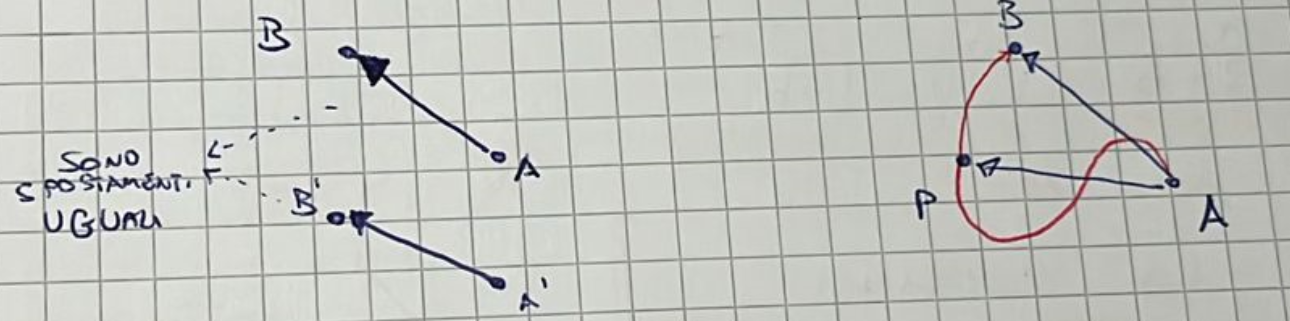
\includegraphics[scale=0.3]{img1.png}

\end{center}
\begin{itemize}
  \item Tutte le grandezze fisiche che si comportano come lo spostamento sono vettori\\Notazioni vettoriali\\\begin{tabular}{cc}
          \textbf{Vettore} & \textbf{Modulo} \\
          {AB}             & $\overline{AB}$ \\
          v                & v               \\
          $\vec{V}$        & $|\vec{V}|$
        \end{tabular}
\end{itemize}
\section{Somma di vettori: Metodo grafico}

$\vec{A}+\vec{B}=\vec{s}$\\
\underline{non} è la somma dei moduli\\
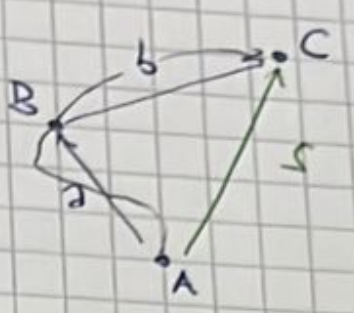
\includegraphics[scale=0.3]{img2.png}

Proprietà della somma
\begin{itemize}
  \item Commutativa: $\vec{a}+\vec{b}=\vec{b}+\vec{a}$
  \item Associativa: $(\vec{a}+\vec{b})+\vec{c}=\vec{a}+(\vec{b}+\vec{c})$\\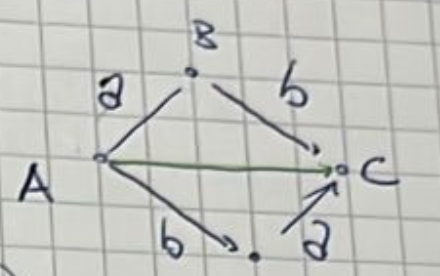
\includegraphics[scale=0.3]{img3.png}
\end{itemize}
\section{Sottrazione}
Il vettore $-\vec{b}$ ha la stessa intensità di $\vec{b}$, ma verso opposto\\
La differenza è la somma di $\vec{a}$ e $-\vec{b}$\\
$\vec{a}-\vec{b}=\vec{a}+(-\vec{b})$\\
\section{Componenti dei vettori}
Proietto le componenti sull'asse delle x\\
$a_x=a\cos\theta$\\
$a_y=a\sin\theta$\\
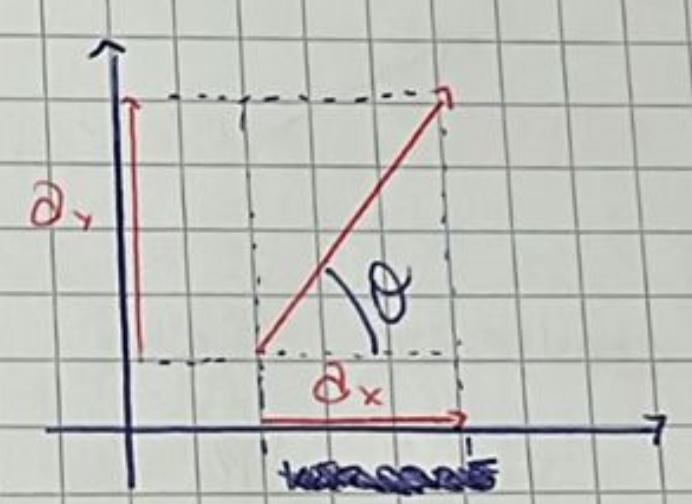
\includegraphics[scale=0.3]{img4.png}
Le componenti:
\begin{itemize}
  \item Sono scalari
  \item Insieme definiscono in modo univoco il vettore\\$|a|=\sqrt{a_x^2+a_y^2}$\\$\tan\theta=\frac{a_y}{a_x}$
\end{itemize}
\section{Versori}
\begin{definition}
  Un \textbf{versore} è un vettore con modulo=1
\end{definition}
\begin{figure}[!ht]
  \centering
  \resizebox{0.5\textwidth}{!}{%
    \begin{circuitikz}
      \tikzstyle{every node}=[font=\LARGE]
      \draw [->, >=Stealth] (8,10.75) -- (13.25,10.75);
      \draw [->, >=Stealth] (8,10.75) -- (8,15.25);
      \draw [->, >=Stealth] (8,10.75) -- (5,8.25);
      \draw [ color={rgb,255:red,255; green,0; blue,0}, ->, >=Stealth] (8,10.75) -- (6.5,9.5);
      \draw [ color={rgb,255:red,255; green,0; blue,0}, ->, >=Stealth] (8,10.75) -- (9.75,10.75);
      \draw [ color={rgb,255:red,255; green,0; blue,0}, ->, >=Stealth] (8,10.75) -- (8,12.5);
      \node [font=\LARGE, color={rgb,255:red,255; green,0; blue,0}] at (8.5,11.75) {k};
      \node [font=\LARGE, color={rgb,255:red,255; green,0; blue,0}] at (8.75,10.25) {j};
      \node [font=\LARGE, color={rgb,255:red,255; green,0; blue,0}] at (7,10.75) {i};
    \end{circuitikz}
  }%
  \label{fig:my_label}
\end{figure}
i, j, k sono i versori della terna cartesiana destrorsa\\
Si indicano anche con $\hat{i}, \hat{j}, \hat{k}$\\
\begin{figure}[!ht]
  \centering
  \resizebox{0.5\textwidth}{!}{%
    \begin{circuitikz}
      \tikzstyle{every node}=[font=\normalsize]
      \draw [->, >=Stealth] (8,10.75) -- (13.25,10.75);
      \draw [->, >=Stealth] (8,10.75) -- (8,15.25);
      \draw [->, >=Stealth] (8,10.75) -- (5,8.25);
      \draw [ color={rgb,255:red,0; green,255; blue,145}, ->, >=Stealth] (8,10.75) -- (6.5,9.5);
      \draw [ color={rgb,255:red,0; green,255; blue,145}, ->, >=Stealth] (8,10.75) -- (9.75,10.75);
      \draw [ color={rgb,255:red,0; green,255; blue,145}, ->, >=Stealth] (8,10.75) -- (8,12.5);
      \node [font=\normalsize, color={rgb,255:red,0; green,255; blue,145}] at (7,10.25) {$a_x$};
      \draw [->, >=Stealth] (8,10.75) -- (8.25,9.5);
      \draw [ color={rgb,255:red,255; green,0; blue,0}, ->, >=Stealth] (8,10.75) -- (8.25,11.25);
      \draw [dashed] (6.5,9.5) -- (8.25,9.5);
      \draw [dashed] (9.75,10.75) -- (8.25,9.5);
      \node [font=\normalsize, color={rgb,255:red,0; green,255; blue,145}] at (9.25,11) {$a_y$};
      \node [font=\normalsize, color={rgb,255:red,0; green,255; blue,145}] at (7.75,12) {$a_z$};
      \draw [dashed] (8.25,9.5) -- (8.25,11.25);
      \draw [dashed] (8,12.5) -- (8.25,11.25);
      \node [font=\normalsize, color={rgb,255:red,255; green,0; blue,0}] at (8,11) {$a$};
    \end{circuitikz}
  }%


\end{figure}\\
$\vec{a}=a_x\hat{i}+a_y\hat{j}+a_z\hat{k}$\\
$\vec{a}$ si può scrivere con: $\vec{a}=(a_x, a_y, a_z)$\\
\section{Somma di vettori: metodo delle componenti}
$\vec{r}=\vec{a}+\vec{b}$\\
$r_x\hat{i}+r_y\hat{j}+r_z\hat{k}=(a_x\hat{i}+a_y\hat{j}+a_z\hat{k})+(b_x\hat{i}+b_y\hat{j}+b_z\hat{k})=\\=(a_x+b_x)\hat{i}+(a_y+b_y)\hat{j}+(a_z+b_z)\hat{k}$\\
$r_x=(a_x+b_x)$\\
$r_y=(a_y+b_y)$\\
$r_z=(a_z+b_z)$\\
\section{Prodotto di vettori}
\subsection{Prodotto tra vettore e scalare}
Scalare = c\\
Vettore = $\vec{a}$\\
Il prodotto dà:
\begin{itemize}
  \item Modulo $|a|*c$
  \item Direzione di $\vec{a}$
  \item Verso di $\vec{a}$ se c$>$0, opposto se c$<$0
\end{itemize}
\subsection{Prodotto tra vettore e vetttore}
$\vec{a}*\vec{b}$\\
$=|a|*|b|*\cos\theta$\\
\begin{figure}[!ht]
  \centering
  \resizebox{0.3\textwidth}{!}{%
    \begin{circuitikz}
      \tikzstyle{every node}=[font=\large]

      \draw [->, >=Stealth] (7,8.5) -- (9.5,11.25);
      \draw [->, >=Stealth] (7,8.5) -- (10.5,8.5);
      \draw [ color={rgb,255:red,0; green,255; blue,110} ] (7,8.5) circle (0.75cm);
      \node [font=\large, color={rgb,255:red,27; green,255; blue,125}] at (8,9) {$\theta$};
      \node [font=\large] at (8.5,8.25) {b};
      \node [font=\large] at (8,10) {a};
    \end{circuitikz}
  }%


\end{figure}
$\vec{a}*\vec{b}$ si può pensare come\\
a * proiezione di b su a\\
$a*(cos\theta b)$ e viceversa\\
\begin{itemize}
  \item Quando i vettori sono perpendicolari il prodotto scalare è 0 (il coseno è 0)\\$\hat{i}*\hat{k}=\hat{k}*\hat{j}=\hat{j}*\hat{i}=0$
  \item Quando i vettori sono paralleli il coseno è 1 e si ha $a*b=|a|*|b|$
  \item $\vec{a}*\vec{b}=(a_x\hat{i}+a_y\hat{j}+a_z\hat{k})*(b_x\hat{i}+b_y\hat{j}+b_z\hat{k})=a_xb_x+a_yb_y+a_zb_z$
  \item Il coseno dell'angolo tra i 2 vettori:\\$\cos\theta=\frac{\vec{a}*\vec{b}}{ab}=\frac{a_xb_x+a_yb_y+a_zb_z}{ab}$
\end{itemize}
\subsection{Prodotto vettoriale}
$\vec{c}=\vec{a}\times\vec{b}$ (``a vettor b'')\\
\begin{itemize}
  \item Modulo $c=|\vec{a}\times\vec{b}|=ab\sin\theta$
  \item Direzione: perpendicolare al piano individuato da $\vec{a}$ e $\vec{b}$
  \item Verso: regola della mano destra
        \begin{figure}[!ht]
          \centering
          \resizebox{0.3\textwidth}{!}{%
            \begin{circuitikz}
              \tikzstyle{every node}=[font=\large]

              \draw [->, >=Stealth] (9.5,9) -- (9.5,11.5);
              \draw [->, >=Stealth] (9.5,9) -- (12,9);
              \draw [->, >=Stealth] (9.5,9) -- (8.25,7.75);
              \node [font=\large] at (11.25,8.5) {$a$};
              \node [font=\large] at (7.75,8.25) {$a \times b$};
              \draw [->, >=Stealth] (7.25,8.5) -- (7.75,8.5);
              \draw [->, >=Stealth] (8,8.5) -- (8.5,8.5);
              \node [font=\large] at (10,11.25) {$b$};
              \draw [->, >=Stealth] (9.75,11.5) -- (10.25,11.5);
              \draw [->, >=Stealth] (11,8.75) -- (11.5,8.75);
            \end{circuitikz}
          }%


        \end{figure}
        \\$(\vec{a}\times\vec{b})=-(\vec{b}\times\vec{a}) \Rightarrow $ non è commutativa
  \item Due vettori paralleli danno prodotto vettoriale = 0\\$\hat{i}\times\hat{i}=0 ...$
  \item Mentre $\hat{i}\times\hat{j}=\hat{k} (\hat{j}\times\hat{i}=-\hat{k})$\\$\hat{j}\times\hat{k}=\hat{i} (\hat{k}\times\hat{j}=-\hat{i})$\\$\hat{k}\times\hat{i}=\hat{j} (\hat{i}\times\hat{k}=-\hat{j})$
  \item Con le \underline{componenti cartesiane}\\
        $\vec{a}\times\vec{b}=(a_x\hat{i}+a_y\hat{j}+a_z\hat{k})\times(b_x\hat{i}+b_y\hat{j}+b_z\hat{k})$\\$=(a_yb_z-a_zb_y)\hat{i}+(a_zb_x-a_xb_z)\hat{j}+(a_xb_y-a_yb_x)\hat{k}$\\
          Può essere ricordato facilmente col determinante\\\\
        $\vec{a}\times\vec{b}=\begin{vmatrix}
          \hat{i} & \hat{j} & \hat{k} \\
          a_x     & a_y     & a_z     \\
          b_x     & b_y     & b_z     \\
        \end{vmatrix}=\hat{i}(a_yb_z-a_zb_y)-\hat{j}(a_xb_z-a_zb_x)+\hat{k}(a_xb_y-a_yb_x)$
  \item La divisione non è definita
\end{itemize}
Esercizi
\begin{enumerate}
  \item Mostrare che $\vec{A}$ è perpendicolare a $\vec{B}$ se $|\vec{A}+\vec{B}|=|\vec{A}-\vec{B}|$\\
        Somma $\vec{S}=(A_x+B_x)\hat{i}+(A_y+B_y)\hat{j}+(A_z+B_z)\hat{k}$\\
        Differenza $\vec{D}=(A_x-B_x)\hat{i}+(A_y-B_y)\hat{j}+(A_z-B_z)\hat{k}$\\
        $(A_x+B_x)^2+(A_y+B_y)^2+(A_z+B_z)^2=(A_x-B_x)^2+(A_y-B_y)^2+(A_z-B_z)^2$\\
        Svolgo i quadrati e ottengo\\
        $(A_x+B_x)+(A_y+B_y)+(A_z+B_z)=0$\\
        $\Rightarrow \vec{A}* \vec{B}=0$ quindi i vettori sono perpendicolari
  \item Calcolare l'angolo compreso tra $a=2\hat{i}-2\hat{j}+5\hat{k}$ e $b=2\hat{i}+\hat{j}-4\hat{k}$

        \begin{figure}[!ht]
          \centering
          \resizebox{0.3\textwidth}{!}{%
            \begin{circuitikz}
              \tikzstyle{every node}=[font=\large]
              \draw [->, >=Stealth] (9.5,9) -- (9.5,11.5);
              \draw [->, >=Stealth] (9.5,9) -- (12,9);
              \draw [->, >=Stealth] (9.5,9) -- (8.25,7.75);
              \node [font=\large, color={rgb,255:red,0; green,255; blue,17}] at (9,9.75) {$a$};
              \node [font=\large, color={rgb,255:red,255; green,0; blue,0}] at (9.75,8.5) {$b$};
              \draw [ color={rgb,255:red,0; green,255; blue,17}, ->, >=Stealth] (9.5,9) -- (8.25,9.75);
              \draw [ color={rgb,255:red,255; green,0; blue,0}, ->, >=Stealth] (9.5,9) -- (9.25,8);
            \end{circuitikz}
          }%

        \end{figure}

        Dalla definizione $\vec{a}*\vec{b}=|a|*|b|*\cos\theta$\\
        Ma vale anche $\vec{a}*\vec{b}=a_xb_x+a_yb_y+a_zb_z$\\
        $\cos\theta=\frac{a_xb_x+a_yb_y+a_zb_z}{a*b}$\\
        $a=\sqrt{2^2+(-2)^2+5^2}=\sqrt{4+4+25}=\sqrt{33}$\\
        $b=\sqrt{2^2+1^2+3^2}=\sqrt{4+1+9}=\sqrt{14}$\\
        $\cos\theta=\frac{2*2+(-2)*1+5*(-4)}{\sqrt{33}*\sqrt{14}}=-0,605 \Rightarrow \theta=127,12^{\circ}$
  \item Prodotto vettoriale tra $\vec{a}=3\hat{i}+7\hat{j}$ e $\vec{b}=2\hat{i}-5\hat{j}$\\
        $\vec{a}\times\vec{b}=\begin{vmatrix}
            \hat{i} & \hat{j} & \hat{k} \\
            3       & 7       & 0       \\
            2       & -5      & 0
          \end{vmatrix}=-29\hat{k}$
\end{enumerate}
\section{Moto in due e tre dimensioni}
Cinematico in più dimensioni\\
\textbf{Vettore posizione}\\
Ha la coda nell'origine e la punta dove c'è la particella\\
$\vec{r}=x\hat{i}+y\hat{j}+z\hat{k}$\\
\begin{figure}[!ht]
  \centering
  \resizebox{0.2\textwidth}{!}{%
    \begin{circuitikz}
      \tikzstyle{every node}=[font=\large]
      \draw [short] (10.5,12.75) -- (10.5,9.75);
      \draw [short] (8.25,11.25) -- (12,11.25);
      \draw [short] (12,12.75) -- (9,9.75);
      \draw  (8.75,10.75) circle (0cm);
      \node at (9,10.75) [circ] {};
      \node [font=\large] at (8.5,10.5) {$P$};
      \draw [ color={rgb,255:red,255; green,0; blue,0}, ->, >=Stealth] (10.5,11.25) -- (9,10.75);
    \end{circuitikz}
  }%

\end{figure}
\vspace{0.1cm}

\textbf{Spostamento}\\
$\Delta\vec{r}=\vec{r_2}-\vec{r_1}$\\
$\Delta r$ è il vettore che va da $r_1$ a $r_2$\\
\begin{figure}[!ht]
  \centering
  \resizebox{0.2\textwidth}{!}{%
    \begin{circuitikz}
      \tikzstyle{every node}=[font=\large]
      \draw [->, >=Stealth] (9.75,9) -- (9.75,11.25);
      \draw [->, >=Stealth] (9.75,9) -- (12,9);
      \draw [->, >=Stealth] (9.75,9) -- (8.25,7.75);
      \node at (8.25,9) [circ] {};
      \node at (10.5,8) [circ] {};
      \draw [short] (8.25,9) -- (10.5,8);
      \draw [short] (8.25,9) -- (9.75,9);
      \draw [short] (10.5,8) -- (9.75,9);
      \node [font=\large] at (8.25,9.5) {$r_1$};
      \node [font=\large] at (11,8) {$r_2$};
      \node [font=\large] at (9.25,8) {$\Delta r$};
    \end{circuitikz}
  }%

\end{figure}
\vspace{0.1cm}
\begin{property}
  Si scrive $\Delta r=(x_2\hat{i}*y_2\hat{j}*z_2\hat{k})-(x_1\hat{i}*y_1\hat{j}*z_1\hat{k})=\Delta x\hat{i}+\Delta y\hat{j}+\Delta z\hat{k}$
\end{property}
\subsection{Velocità vettoriale media e istantanea}
\textbf{Media}\\
Rapporto tra lo spostamento $\Delta r$ nel l'intervallo di tempo $\Delta t$ e l'intervallo stesso\\
$\overline{\vec{v}}=\frac{\Delta \vec{r}}{\Delta t}=\frac{\vec{r_2}-\vec{r_1}}{t_2-t_1}$
\begin{figure}[!ht]
  \centering
  \resizebox{0.2\textwidth}{!}{%
    \begin{circuitikz}
      \tikzstyle{every node}=[font=\large]
      \draw [->, >=Stealth] (8.25,8) -- (8.25,11.5);
      \draw [->, >=Stealth] (7.75,8.5) -- (11.5,8.5);
      \node at (9,10.25) [circ] {};
      \node at (10.5,9.5) [circ] {};
      \draw [short] (9,10.25) -- (10.5,9.5);
      \draw [->, >=Stealth] (8.25,8.5) -- (9,10.25);
      \draw [->, >=Stealth] (8.25,8.5) -- (10.5,9.5);
      \node [font=\large] at (8.5,9.75) {$r_1$};
      \node [font=\large] at (9.75,9) {$r_2$};
      \node [font=\large] at (9,10.75) {$1$};
      \node [font=\large] at (11,9.5) {$2$};
      \node [font=\large, color={rgb,255:red,255; green,0; blue,0}] at (9.75,11) {$\rightarrow$};
      \draw [ color={rgb,255:red,255; green,0; blue,0}, short] (9,10.25) -- (11,10.75);
      \node [font=\large] at (10,10) {$\Delta r$};
      \node [font=\large, color={rgb,255:red,255; green,0; blue,0}] at (9.75,10.75) {$v$};
    \end{circuitikz}
  }%

\end{figure}
\vspace{0.1cm}\\
\textbf{Istantanea}\\
$\vec{v}=\lim_{\Delta t\to0}\frac{\Delta \vec{r}}{\Delta t}=\frac{dr(t)}{dt}$\\
$\vec{v}=\frac{d\vec{r}}{dt}=\frac{dx\hat{i}+dy\hat{j}+dz\hat{k}}{dt}=\frac{dx}{dt}\hat{i}+\frac{dy}{dt}\hat{j}+\frac{dz}{dt}\hat{k}$\\
\subsection{Accelerazione media e istantanea}
\textbf{Media}\\
$\overline{\vec{a}}=\frac{\Delta \vec{v}}{\Delta t}=\frac{\vec{v_2}-\vec{v_1}}{t_2-t_1}$\\\\
\textbf{Istantanea}\\
$\vec{a}=\lim_{\Delta t\to0}\frac{\Delta \vec{v}}{\Delta t}=\frac{d\vec{v}}{dt}=\frac{d^2r}{d^2t}$\\
\end{document}